Both agents use the same DQN training loop, summarized below: replay buffer,
epsilon-greedy exploration, a target network, Adam optimization, and Huber
loss (smooth L1) for the Bellman error. Observations are normalized
before being passed to the Q-network. For CartPole-v1, the four state variables
are scaled by fixed practical bounds and clipped to the interval $[-\pi,\pi]$.

The DQN loop proceeds as follows. After each environment step, the transition
$(s, a, r, s', d)$ is stored in a fixed-capacity replay buffer $\mathcal{D}$.
Once $|\mathcal{D}| \geq \text{learning\_starts}$, a minibatch of $B$
transitions is sampled uniformly from $\mathcal{D}$. The Bellman target is
$y_j = r_j + \gamma (1-d_j) \max_{a'} Q_{\theta^-}(s'_j, a')$ for standard
DQN, or $y_j = r_j + \gamma (1-d_j) Q_{\theta^-}(s'_j, \arg\max_{a'}
Q_\theta(s'_j, a'))$ for Double DQN, where $\theta^-$ denotes the target
network parameters, updated every target\_update steps. The loss is
$\mathcal{L} = \frac{1}{B}\sum_j \text{Huber}(Q_\theta(s_j, a_j), y_j)$,
minimized via Adam with gradient clipping. Exploration follows linear
$\epsilon$-decay from 1.0 to 0.05.

The MLP baseline is a single-hidden-layer network. For the main L1
configuration, it uses 3 hidden units, resulting in 23 trainable parameters.
This intentionally small network was chosen to match the parameter budget of
the VQC. For the Dueling variant, the network trunk feeds two separate heads:
a value head $V(s) \in \mathbb{R}$ and an advantage head $A(s,\cdot) \in
\mathbb{R}^{|\mathcal{A}|}$, which are combined as $Q(s,a) = V(s) + A(s,a)
- \frac{1}{|\mathcal{A}|}\sum_{a'} A(s,a')$.

\subsubsection*{VQC Architecture}

The VQC agent uses 4 qubits, angle encoding with $RY$ gates, one or three
variational layers, and a ring of CNOT gates. Each variational layer applies a
trainable three-parameter rotation $R(\alpha,\beta,\gamma) = RZ(\gamma)RY(\beta)
RZ(\alpha)$ to every qubit. The readout extracts Pauli-Z expectation values
$\langle Z_i \rangle \in [-1,1]$ for all qubits, yielding a 4-dimensional
classical feature vector that is then mapped to Q-values by a linear layer.
The main VQC configuration has $4 \times 3 = 12$ trainable gate parameters plus
$4 \times 2 + 2 = 10$ readout parameters, totaling 22 trainable parameters.
The L3 variant uses three layers ($3 \times 4 \times 3 = 36$ gate parameters)
for 46 total parameters.

\subsubsection*{Batched QNode Optimization}

The original implementation evaluated the QNode once per sample in each
training batch. For a batch of size $B$, this required $B$ separate calls to the
PennyLane QNode, each building a separate automatic differentiation
computation graph. We replaced this with a single batched call using PennyLane
parameter broadcasting: the input tensor of shape $[B, 4]$ is zero-padded to
$[B, 4] \rightarrow [B, 4]$ (no padding needed since $n_{\text{qubits}} = 4$)
and passed to the QNode as $[B, n_{\text{qubits}}]$. The encoding gate
$RY(\text{inputs}[:, i])$ naturally broadcasts across the batch dimension,
producing expectation values of shape $[B, n_{\text{qubits}}]$ in a single
forward pass. This optimization reduced the per-update VQC overhead from
$\mathcal{O}(B)$ QNode calls to $\mathcal{O}(1)$.

\subsubsection*{Exploration and Feature Modes}

The standard exploration policy is $\epsilon$-random. We also tested a
fuzzy-guided exploration variant where, with probability $\epsilon$, the action
is selected by a fixed fuzzy heuristic $a = \mathbf{1}[\theta + 0.25\dot{\theta}
+ 0.01x + 0.01\dot{x} > 0]$ instead of uniformly random. This biases early
exploration towards higher-reward trajectories without affecting the learned
policy evaluation.

Three observation preprocessing modes are supported. \emph{Raw normalized}
scales and clips each state variable. \emph{Fuzzy compact} adds stability and
recommendation scores (not used in main results due to action leakage).
\emph{Fuzzy membership} produces four features: pole falling left/right ($f_1,
f_2$) and cart escaping left/right ($f_3, f_4$), computed as:

\begin{equation}
f_1 = \text{clip}\!\left(\frac{-\theta}{\theta_{\max}} +
\frac{-\dot{\theta}}{\dot{\theta}_{\text{scale}}},\; 0,\; 1\right), \quad
f_2 = \text{clip}\!\left(\frac{\theta}{\theta_{\max}} +
\frac{\dot{\theta}}{\dot{\theta}_{\text{scale}}},\; 0,\; 1\right)
\end{equation}
\begin{equation}
f_3 = \text{clip}\!\left(\frac{-x}{x_{\max}} +
\frac{-\dot{x}}{\dot{x}_{\text{scale}}},\; 0,\; 1\right), \quad
f_4 = \text{clip}\!\left(\frac{x}{x_{\max}} +
\frac{\dot{x}}{\dot{x}_{\text{scale}}},\; 0,\; 1\right)
\end{equation}

These features describe the state's risk profile without encoding a recommended
action.

\subsubsection*{Fuzzy-Teacher Distillation}

In addition to the DQN experiments, we include a separate fuzzy-teacher
distillation experiment. A fixed CartPole balancing heuristic (the linear rule
$a = \mathbf{1}[\theta + 0.25\dot{\theta} + 0.01x + 0.01\dot{x} > 0]$)
labels $N$ uniformly sampled states with a reference action. The small MLP or
VQC is trained as a classifier to imitate this teacher via cross-entropy loss
$\mathcal{L}_{\text{distill}} = -\frac{1}{N}\sum_{i=1}^N
\log P_\theta(a_i^{\text{teacher}} | s_i)$. This experiment uses the same model
architectures (MLP with 3 hidden units, VQC with 4 qubits and 1 or 3 layers)
as the DQN experiments, but substitutes the RL training objective with
supervised policy cloning. We evaluate two input representations: raw
normalized state and fuzzy membership. The purpose is to test whether the same
low-parameter models can represent a useful control policy under an easier
optimization signal, thereby isolating the effect of the training objective
(reward-based DQN vs.\ supervised distillation).

\begin{figure}[t]
  \centering
  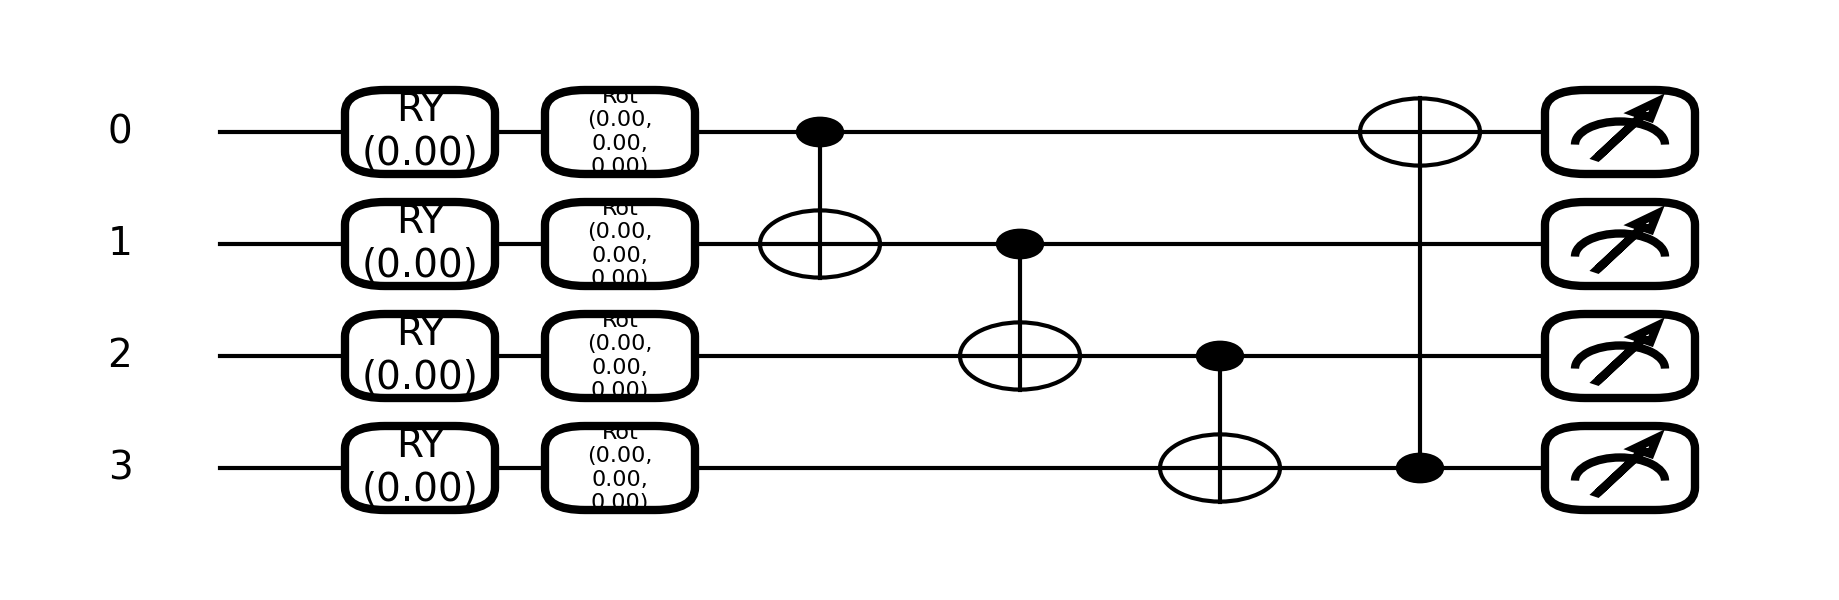
\includegraphics[width=0.95\linewidth]{figures/vqc_l1_circuit.png}
  \caption{VQC architecture with $RY$ angle encoding, 1 layer of $R(\alpha,\beta,\gamma)$ rotations, ring CNOT entanglement, and Pauli-Z readout. Black circles indicate qubits.}
  \label{fig:vqc-circuit}
\end{figure}
